%We have decided to utilize the FP package for doing calculations and tracking constants in the CDR
% (e.g. the limit of annual data from ll active FD modules to permanent storage at FNAL is 30 GB/year)
% The template for a variable is this:
% "chapter""section"variable where both "chapter" and "section" are abbreviations
% with the Camel Caps used for readability
% Note that you should not override the use of a variable defined in generated/parameters.tex

%Start of Introduction variables (Intro)

%End of Introduction varaibles

% Data and Processing Volume Estimates (DatVol)

\FPset{DatVolFDColdElecPrecision}{12} %number of bits in cold electronics digitization

% Use Cases (UseCase)

% Frameworks (Fra)

% Databases (DBs)

% Applications (App)

% Computing Model (CompMod)

% Site Resources (SiteRes)

% Data Placement (DataPla)

% Networking (Net)

% Workflow Examples (Wrkflw)


\chapter{Introduction : (Schellman) }
\label{ch:intro}

%%%%%%%%%%%%%%%%%%%%%%%%%%%%%%%%
\section{xyz}
\label{sec:intro:xyz}  %% fix label according to section

\todo{Need to add discussion of physics requirements that drive computing}

\section{Introduction}

The \dword{dune}  will begin running in the late 2020's.  The goals of the experiment include 1) studying neutrino oscillations using a beam of neutrinos from Fermilab in Illinois to the Homestake mine in Lead, South Dakota, 2) studying  astrophysical neutrino sources and rare processes and 3) understanding  the physics of neutrino interactions in matter.   I will concentrate on the neutrino oscillation and supernova capabilities of the experiment and the ways that they drive computing. 

The neutrino beam from Fermilab will consist almost entirely of muon-type neutrinos when produced.  Neutrinos are known to come in (at least) 3 flavors which can be distinguished by their interactions - electron type neutrinos produce electrons when they interact via charged currents; muon neutrinos, muons; and tau neutrinos, tau particles.  But these flavors do not correspond to fixed mass states.  All 3 flavors of neutrinos are mixtures of mass states, much as  light polarized in the $x$ direction  can be considered a superposition of  $x^\prime$ and $y^\prime$ polarizations along  alternate axes rotated by 45 degrees.  When neutrinos propagate through space, it is the mass state that sets their wavelength and if the neutrino goes far enough, the multiple mass states  corresponding to the initial flavor state will get out of phase.  When the mixture is later probed about its flavor, it  may give a different answer than the neutrino that started out. This phenomenon is neutrino oscillation and has been shown to exist in multiple experiments since it was first confirmed in 1998\cite{Kajita2006}.

\begin{figure}[h]
    \centering
\includegraphics[height=6cm]{graphics/IntroFigures/Fig_01_neutrinos.jpg}
    \caption{Illustration of the neutrino flavor and mass states.  The mass states are a superposition of the flavor states.  Courtesy the particlezoo.net.}
    \label{fig:neutrinos}
\end{figure}

\begin{figure}[h]
    \centering
\includegraphics[trim={0cm 0.6cm 2.5cm 0.7cm},clip,height=6cm]{graphics/IntroFigures/Fig_02_Argoneut.jpg}    \caption{Electron neutrino appearance signal (top) and background (bottom) as seen in the ArgoNeut experiment\protect{\cite{Acciarri:2016sli}}.  In the true appearance signal, an electron is seen emerging from the primary vertex and then showering.  In the background interaction, a muon neutrino enters and  produces a final state muon and photons, which propagate some distance before showering.}
    \label{fig:Argoneut}
\end{figure}

DUNE,  in particular,   wishes to understand the conversion of muon neutrinos created in Illinois into electron neutrinos at a \dword{fd} in the Homestake mine in South Dakota and compare that conversion rate between neutrino and anti-neutrino beams. The location of the \dword{fd} and energy of the neutrino beam were chosen to maximize the oscillation effect.   A difference in the conversion rate for neutrinos and anti-neutrinos could be evidence for matter-antimatter asymmetry in the neutrino sector, a phenomenon called CP violation.  

To make these measurements, we need to be able to distinguish electron neutrino interactions appearing in the muon neutrino beam from the dominant muon neutrino interactions one would expect in the absence of oscillations.  Doing this requires a very large detector, as neutrino interactions are intrinsically rare, but an extremely  fine grained one as well.  Noble liquid time projection detectors, which read out large transparent volumes of liquid by drifting electrons from interactions to charge detectors through strong electric fields, have the needed capabilities of extremely large scale and fine-grained resolution. The proposed DUNE far-site detector will instrument four  $14\times12 \times58$ meter volumes of Liquid Argon with readout granularity of 0.5 cm.  The detectors will be located 4850 ft below the surface to lower the rate of cosmic rays traversing the detector by orders of magnitude and thus allow sensitivity to very low energy solar and astrophysical neutrinos as well as the higher energy neutrinos produced at Fermilab. 




The neutrino beam from Fermilab will be pulsed approximately once/second 24 hrs/day during running periods with of order 15 million pulses per year.  Because neutrinos interact  extremely rarely, we expect to detect of order 7,500  neutrino interactions/year in each of 4 10~kT detector modules located at the \dword{fd} site in South Dakota. 






Construction of the detector halls and infrastructure for the large 10 kT fiducial volume \dword{fd} modules is starting now, as are design and construction of detector readout modules.  A full \dword{tdr} for the program has recently been completed and is available in references \cite{Abi:2020wmh, Abi:2020evt, Abi:2020oxb, Abi:2020loh}.
The  \dword{dune} neutrino oscillation experiment will receive beam late in this decade with commissioning of the data acquisition systems for the first far detector module expected to start in 2025-26.  

\begin{figure}
\centering
\includegraphics[height=0.35\textwidth]{graphics/IntroFigures/Fig_03a_cryostat-scale.png}
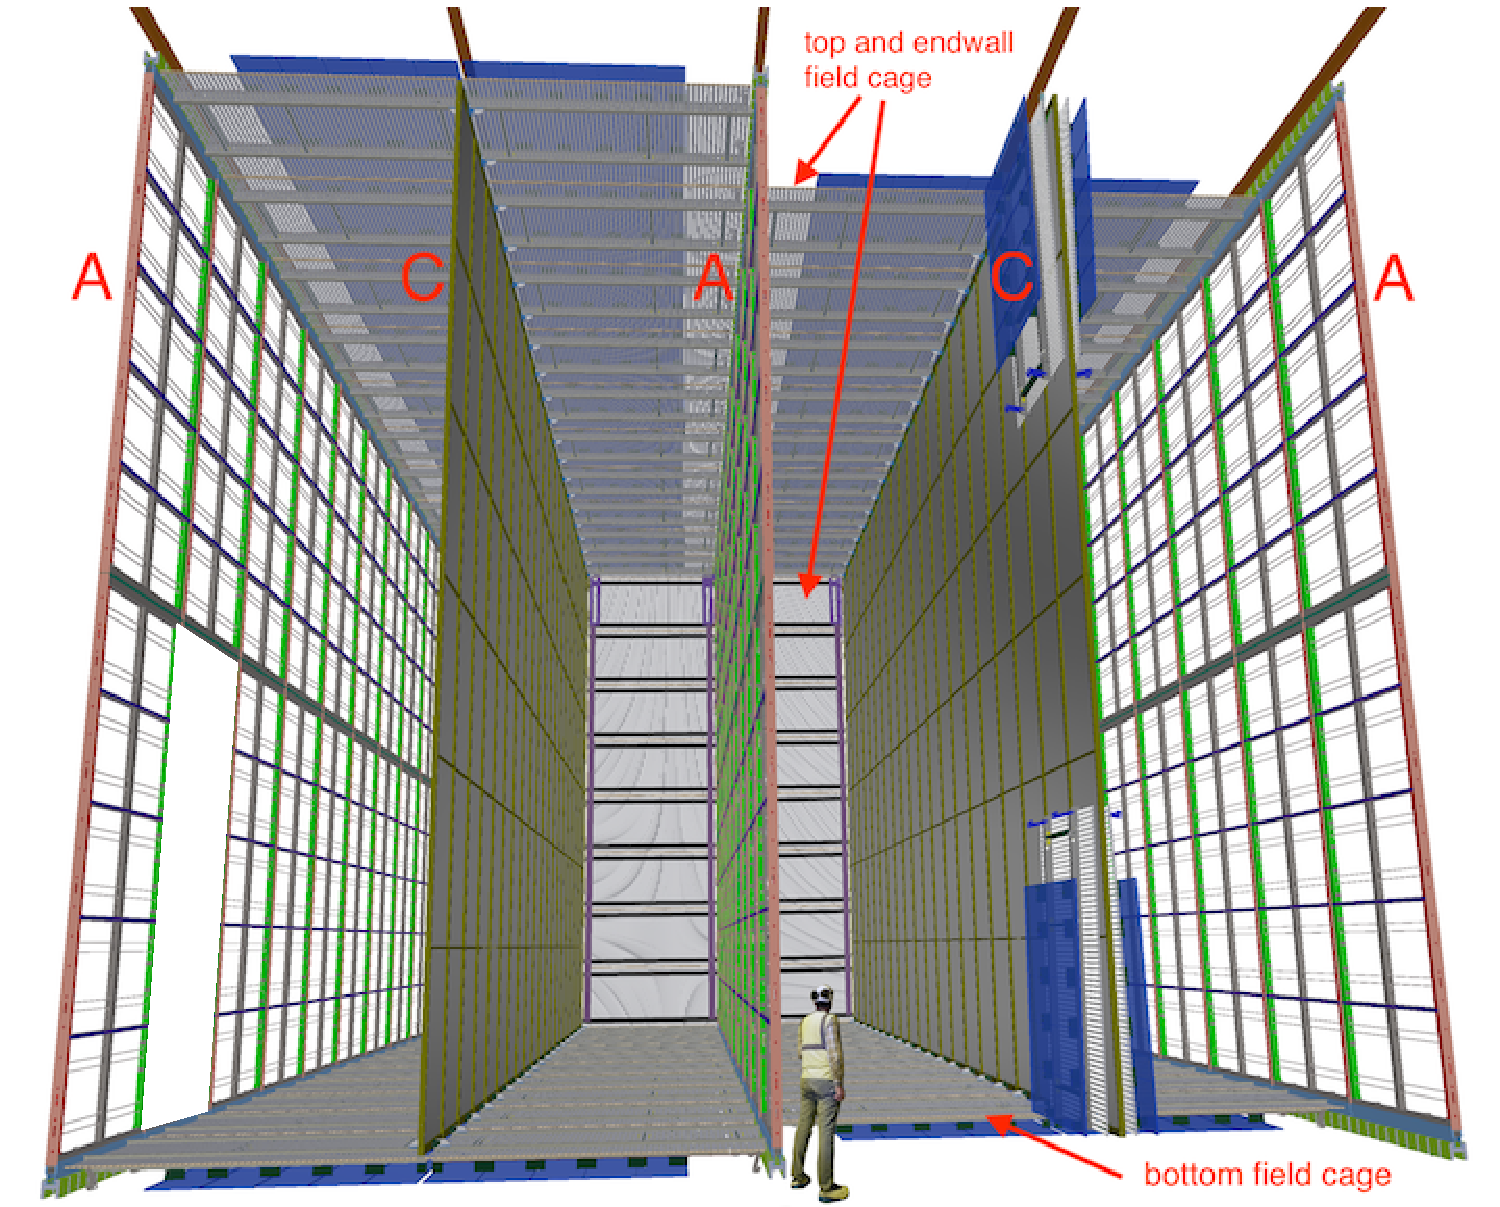
\includegraphics[height=0.35\textwidth]{graphics/IntroFigures/Fig_03b_DUNESchematic.pdf}
\caption{Left) A far detector cryostat that houses a 10 kT \dword{fd} module. The figure of a person indicates the scale.  Right) A 10kt  \dword{dune} \dword{fd} \dword{spmod}, showing the alternating 58 m long (into the page), 12 m high anode (A) and cathode (C) planes, as well as the field cage that surrounds the drift regions between the anode and cathode planes. The blank area on the left side was added to show the profile of a single \dword{apa}.}
\label{DUNESchematic}
\end{figure}

\section{ProtoDUNE tests at CERN}

Building an experiment of this size requires an extensive period of prototyping.   The Argoneut\cite{Acciarri:2018myr}, MicroBooNE\cite{microboone} and ICARUS\cite{icarus} collaborations have demonstrated the capabilities of large liquid Argon \dword{tpc}s for neutrino detection on scales between 1 and 500 ton fiducial mass.  In preparation for the \dword{dune} experiment, a campaign testing proposed DUNE components in 700 ton detectors in the EHN1 hadronic test-beam was launched at CERN in 2018.  Both single-phase and dual-phase prototypes were constructed and tested. % We have tested the full data taking chain from detector construction to full offline reconstruction and analysis of data. 

\subsection{\dword{pdsp}}
The \dword{pdsp} experiment began taking data at CERN in late 2018.  \dword{pdsp} uses single-phase technology where ionization electrons are collected directly from the liquid argon. The readout system consists of  Anode Plane Assemblies (\dword{apa})s which each have 3 layers of wires arranged in different directions. Each layer contains 800-1200  wires spaced 0.5 cm apart. Electrons drift from the original interaction in the Argon, through a strong electric field, to the wire planes and induce signals.  The location in the plane of hit wires gives one coordinate, the time the signal takes to drift to the wire from the original interaction measures a second coordinate.  The third coordinate is derived by combining information from overlaps of signals in the 3 different wire layers.  Signals are amplified electronically and then digitized.  Figure \ref{tpcconcept} illustrates the operation of a generic \dword{lartpc}.

\begin{figure}[h]
    \centering
%    \subfloat[EM]{\label{Blob1_const}
\includegraphics[trim={0cm 0.6cm 2.5cm 0.7cm},clip,height=8cm]{graphics/IntroFigures/Fig_04_LArTPC_Concept.png}%\includegraphics[trim={1.3cm 0.6cm 2.5cm 0.7cm},clip,height=3.5cm]{h_ptmumichel_1track_const_.pdf}
    \caption{Diagram  from  \protect{\cite{ Acciarri:2017sde}}  illustrating the signal formation in a LArTPC with three wire planes~\cite{Acciarri:2016smi}. For simplicity, the signal in the first U induction plane is omitted in the illustration. }%Planes are positioned in the order U, V, Y with the Y plane being farthest from the cathode plane}
    \label{tpcconcept}
    \end{figure}

The \dword{pdsp} detector consists of a 700 ton volume of liquid argon with a cathode plane in the center and 3 \dword{apa}s mounted on  each  edge of the liquid volume.  The drift distance is  3 m with  a nominal voltage of 180kV  across that distance.  Each \dword{apa} has 2560 channels and each channel reads out a 12-bit \dword{adc} every 0.5 $\mu$sec.   For \dword{pdsp} the readout time appropriate for a 3 m drift was set to 3 msec, resulting in 6000 12-bit samples per channel.  The total data size for six \dword{apa}s is thus 140 MB with additional header and data from photon and external tagging systems bringing the nominal event size up to around 180 MB.  Lossless compression of the \dword{tpc} readout was implemented in the data acquisition system, resulting in a final compressed event size of around 75 MB. 

The test-beam ran at rates of up to 25 Hz over a period of 6 weeks at beam momenta between 0.5 and 7 GeV/c.  Time of flight and Cherenkov counters provided beam flavor tagging.  Around 8M total `physics' events were written, with around 3M having beam tag information.  In total  850 TB of raw test-beam data were written, along with one PB of commissioning and cosmic data. These data were successfully cataloged and written to storage at both CERN and Fermilab at rates of up to 2 GB/sec.   

Thanks to significant prior effort in the \dword{lar} computing and algorithms community, reconstruction software was ready to go and the first reconstruction pass began soon after data taking started and was complete within two weeks of the end of data taking.  Those results were extremely useful in demonstrating the capabilities of the detector and summarized in Volume II of the \dword{tdr}\cite{Abi:2020evt}.  A second pass, with improved treatment of instrumental effects ranging from stuck bits to 2-D deconvolution to correction for space charge effects was completed in late 2019. 
%\dword{pdsp} Reconstruction - from raw data to beam interactions and cosmics full reconstructed with 80-90\% efficiency - has been performed twice over the 8M interactions recorded during the test-beam runs. 
Figure \ref{deconvolution} illustrates the signal processing stage of reconstruction, where raw ADC signals have noise and stuck bits removed and are then deconvoluted to yield gaussian hit candidates. Figures \ref{wire-cell-bee} and \ref{pandora} illustrate full pattern recognition and event reconstruction. 

While \dword{lartpc}s benefit from fine granularity and a uniform detector medium, diffusion, argon purity, fluid flow and the build up of space charge in the active medium can all introduce distortions into the detector response.  These effects have all been simulated and tested in the \dword{pdsp} data. 

Compressed raw input event records were of order 75 MB in size and took 500-600 seconds to reconstruct, of which around 180 sec was signal processing and the remainder high level reconstruction dominated by 40-60 cosmic rays per readout.  Memory footprints ranged between 2.5 and 4 GB.  Output event  record sizes were reduced to 22 MB by dropping the raw waveforms after hit finding.   Reconstruction campaigns took of order 4-6 weeks (similar to the original data taking) and utilized up to 15,000 cores on \dword{osg} and \dword{wlcg} resources.  Job submission was done through the POMS\cite{poms} job management system developed at Fermilab. POMS supports submissions to FNAL dedicated resources and selected OSG and WLCG sites.  Figure \ref{sites} shows the distribution of wall hours used for reconstruction in 2019. 

For reconstruction, data were streamed via {\tt xrootd}\cite{Behrmann:2011zz} from {dcache} storage at Fermilab to the remote sites. Despite individual processing jobs taking 15-30 hrs to complete, network interruptions rarely caused job failures. 


 

\begin{figure}[ht]
\centering
%[Raw  and deconvolved induction U-plane signals from a ProtoDUNE-SP event]
%{pDUNE_sp_example}
\includegraphics[width=0.49\textwidth]{graphics/IntroFigures/Fig_05a_protodune_raw_u.pdf}
\includegraphics[width=0.49\textwidth]{graphics/IntroFigures/Fig_05b_protodune_decon_u.pdf}
\caption{Comparison of raw (left) and deconvolved induction U-plane signals (right) before and after 
the signal processing procedure from a \dword{pdsp} event. The bipolar shape with red (blue) color representing
positive (negative) signals is converted to the unipolar shape after the \twod deconvolution.}
\label{deconvolution}
\end{figure}

\begin{figure}
%[\threed display of interaction in ProtoDUNE-SP]
\centering
\includegraphics[width=0.9\textwidth]{graphics/IntroFigures/Fig_06_bee_event.png}
\caption {The \dword{pdsp} detector (gray box) showing 
the direction of the particle beam (yellow line on the very far left) and the outlines of the six \dword{apa}s. Cosmic rays
can be seen throughout the white box, while the red box highlights the beam region of interest with an interaction of the 7 GeV beam. 
The \threed points are obtained using the Space~Point~Solver reconstruction algorithm. }
\label{wire-cell-bee}
\end{figure}

\begin{figure}
\centering
\includegraphics[width=0.8\textwidth]{graphics/IntroFigures/Fig_07_pandora.png}
\caption{Pandora \protect{\cite{Acciarri:2017hat}} reconstruction of cosmic rays and beam interaction in a \dword{pdsp} event. The left side of the figure shows the full detector volume with all interactions, including cosmic rays and the right side shows the identified beam interaction.}
\label{pandora}
\end{figure}


\begin{figure}
\begin{center}
%\includegraphics[height=0.5\textwidth]{Fig_08a_Picture1.png}
%\includegraphics[height=0.5\textwidth]{Fig_08b_Picture2.png}
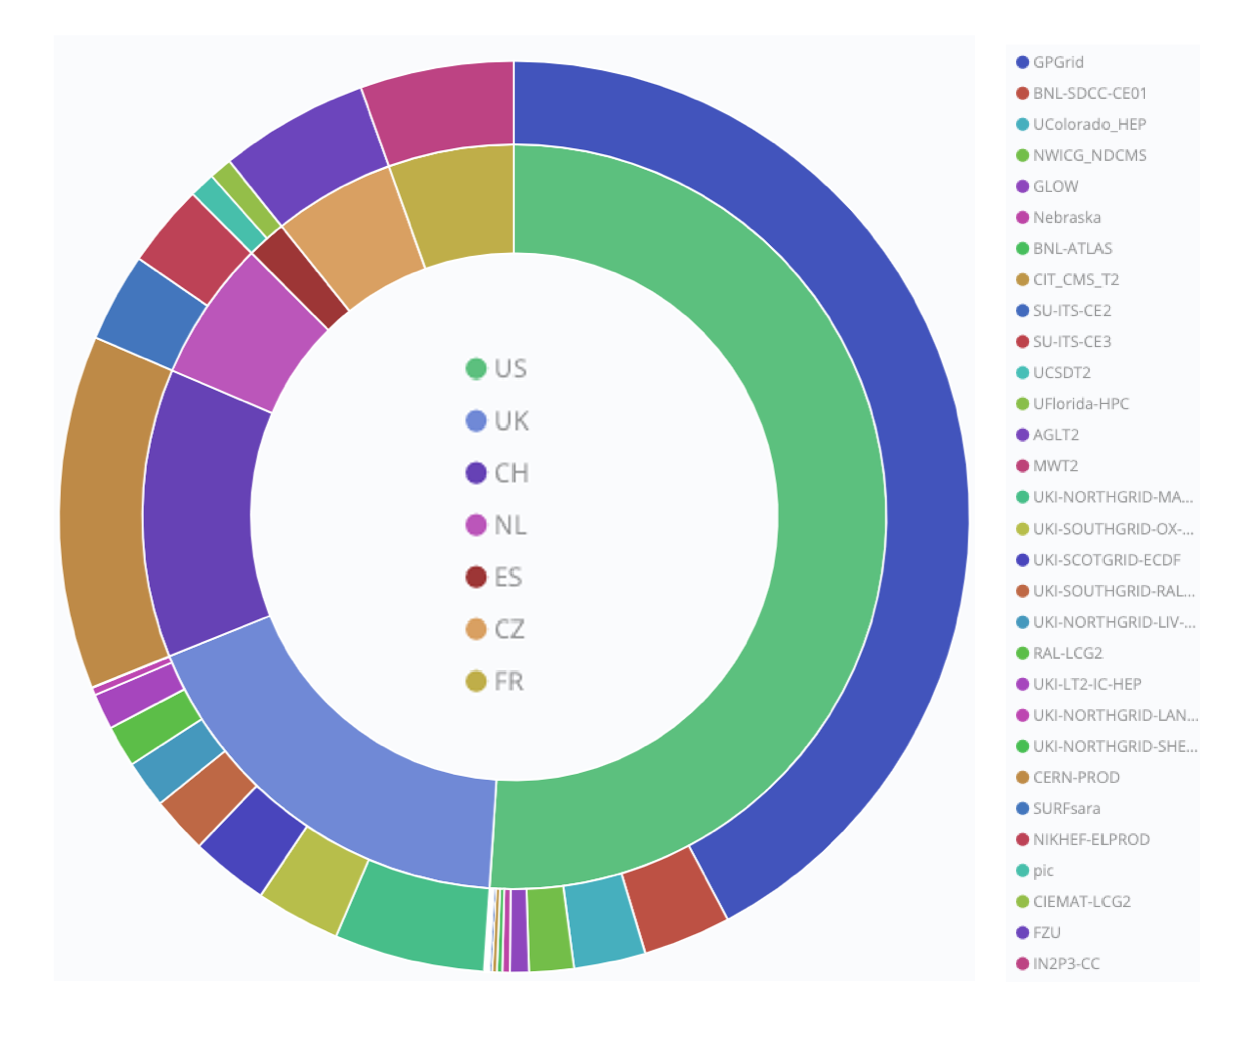
\includegraphics[height=0.65\textwidth]{graphics/IntroFigures/Fig_8.pdf}
\caption{Reconstruction processing distribution amongst sites for DUNE production in calendar 2019.  The inner circle shows national contributions while the outer circle shows individual site contributions.}
\label{sites}
\end{center}
\end{figure}

\subsection{\dword{pddp}}

The \dword{pddp} detector began taking data using cosmic rays in August 2019.  Thanks to preceding data challenges, those data have been successfully integrated into the full data cataloging and reconstruction chains and are now being reconstructed as they arrive.   The \dword{pddp} technology locates the readout systems above a thin layer of argon gas above the liquid argon surface.  This gas layer allows an external electric field to accelerate the electrons and produce gas amplification.  The result is a substantial increase in signal-to-noise in the resulting signals, at the cost of longer electron drifts from the bottom of the liquid volume.  Figure \ref{dpevent} illustrates early data from \dword{pddp}. 

\begin{figure}
\centering
\includegraphics[width=0.85\textwidth]{graphics/IntroFigures/Fig_09_protodune-dp-event.png}
\caption {Cosmic ray data from the dual phase prototype}
\label{dpevent}
\end{figure}


\subsection{Conclusions from prototype tests}
\dword{protodune} prototype runs are ongoing and will continue through beam tests in 2021-22 at \dword{cern}.  Data cataloging, movement and storage techniques were tested before the start of the \dword{pdsp} and \dword{pddp}  runs and were able to handle the full rate of the experiments.   Reconstruction algorithms were also in place on time and were able to produce early results that led to increased understanding of the detector and improved calibrations for a second iteration.  These tests also identified some deficiencies in our infrastructure, including incomplete schemes for the transmission of configuration and conditions information between hardware operations and  offline computing.  The test-beam runs have been extremely valuable in allowing us to determine which variables are important to transmit and in designing improved systems for gathering and storing that information. 

An additional run of both \dword{pdsp} and \dword{pddp} is planned for 2021 and 2022, allowing further developing and testing of our computing infrastructure before the full detector comes online in the late 2020's. 


\section{On to full DUNE}

The full DUNE \dword{fd} will begin with one single phase module to be installed at Homestake starting in the middle of  this decade.  High intensity neutrino and anti-neutrino beams should arrive after a year or so of commissioning of the detector and \dword{lbnf} beamline.  This first module will largely resemble a scaled up version of \dword{pdsp} with 150 \dword{apa}s distributed 2-deep at the center and long edges of the cryostat.   The argon volume will be $15\times14\times62$ m$^3$ with a fiducial mass of 10kT.  Table \ref{tab:volumes} summarizes the expected event rates and data volumes for one such detector module.  Additional detector modules, likely one dual-phase, another single-phase and  one with novel technology will be added.  For now, we assume that data volumes and rates coming from other technologies will be less than or equal to the single-phase values. 



The detectors should be sensitive to neutrino interactions and radioactive decays above an energy threshold of order 5 MeV.  Unambiguous triggering may require a somewhat higher threshold  to avoid false triggers due to $^{39}$Ar decays,  but beam interactions in the 500-10,000 MeV range should have almost perfect detection efficiency. Sophisticated triggering algorithms should also allow standalone detection of astrophysical sources, including higher energy solar neutrinos and supernova candidates. 

The data rates will be dominated by 4,500 cosmic rays expected per module/day.  These events are vital for monitoring and aligning the detector.  The next most significant source of events will be calibration campaigns with radioactive and neutron sources and lasers.  In all cases, the goal is to gather data from the full volume of the detector with as fine a granularity as possible. 

Beam interactions themselves are expected to be quite rare, occurring in only 1/2000 beam gates.  Extraction of oscillation parameters will require both the powerful electron background rejection, discussed in the previous section,  and precise calibration of the energy scale of the experiment, hence the much larger calibration samples. 

 \begin{dunetable}
[Data Sizes and Rates]
{l |r r r }
{tab:volumes}
{Data sizes and rates for different processes in each far detector module.  Uncompressed data sizes are given. As readouts will be self-triggering an extended 5.4 ms readout window is used instead of the 3ms for the triggered \dword{pdsp} runs.  We assume beam uptime of 50\% and 100\% uptime for non-beam science. These numbers are derived from references \protect{\cite{bib:docdb16028}}and \protect{\cite{bib:docdb14983}}.}
5
Process & Rate/module & \qquad size/instance &\qquad  size/module/year\\ \toprowrule
%
Beam event & 41/day & 6 GB&47 TB/year\\
Cosmic rays &4,500/day&  6 GB& 9.7 PB/year\\
Supernova trigger& 1/month& 115 TB& 1.4 PB/year\\
Calibrations&2/year&750 TB& 1.5 PB/year\\
%\toprowrule 
Total& & &12.9 PB/year\\
\end{dunetable}


Overall, bottoms-up estimates yield data volumes of around 13 PB/year/module.  Lossless compression should reduce this volume and additional modules will likely increase these rates.  A maximum rate of 30PB/year across all modules and modes of operation has been specified.  We will note that 30 PB/year is  an average of 1.3 GB/sec, less than the rates already demonstrated for protoDUNE acquisition and storage.  In principle, at 2.5 CPU sec/MB of compressed input, 2000-3000 cores could keep up with these data rates  but this throughput must be maintained over many years.   In addition, supernova candidates may require bursts of  much higher acquisition and processing rates. Table \ref{tab:exec-comp-bigpicture-es} summarizes the computational characteristics expected for \dword{fd} data. 


\subsection{Supernova candidates}


\begin{figure}
\begin{center}
\includegraphics[height=0.3\textwidth]{graphics/IntroFigures/Fig_10a_Picture3.png} \hskip 1 in
\includegraphics[height=0.5\textwidth]{graphics/IntroFigures/Fig_10b_Picture4.png}
\caption{Left) a charged current interaction of a 30 MeV energy electron neutrino in the DUNE Far Detector.  Right) a neutral current excitation and de-excitation of an Ar nucleus by a  10 MeV neutrino.}
\label{blips}
\end{center}
\end{figure}


Supernova candidates pose a unique problem for data acquisition and reconstruction.  Supernova physics in DUNE is discussed in some detail in the \dword{tdr}\cite{ Abi:2020evt} and only summarized here. A classic core-collapse supernova 10 kpc away would be expected to yield around 3,000  charged-current electron neutrino interactions across 4 detector modules.  The oscillation physics is not fully understand and can result in significant modulations of the event rates for different neutrino types  over the few tens of seconds of the burst.  DUNE's fine-grained tracking should allow significant pointing power with the most optimistic scenario of four modules and high electron neutrino fraction yielding pointing resolutions of less than 5 degrees.   Figure \ref{blips} illustrates simulated signatures of supernova neutrino interactions in the far detector. The ability to produce a reasonably fast pointing signal would be extremely valuable to optical astronomers doing followup, especially if a supernova was in a region where dust masks the primary optical signal.   The need to be alert to supernovae and to quickly transfer and process the data imposes significant requirements on triggering, data transfer and reconstruction beyond those imposed by the more regular beam-based oscillation physics.   For example, a compressed supernova readout of all four modules will be of order 184 TB in size and take a minimum of 4 hrs to transfer over a 100 Gbs network,  and then take of order 130,000 CPU-hrs for signal processing at present speeds.  If processing takes the same time as transfer, a peak of 30,000 cores would be needed. 


\fixme{Move or copy to the data volumes section}
\begin{dunetable}
[Useful FD Data Quantities]
{|l  l |c       | l |}
{tab:exec-comp-bigpicture-es}
{Useful quantities for computing estimates for \dword{sp}
readout. For  sparse \dword{fd} events, the pattern recognition phase, which scales with occupancy is expected to be substantially faster than the signal processing phase which scales with detector size.  }%
Quantity&&\qquad Value \qquad&Explanation\qquad \qquad\\
\toprowrule
{\bf Far Detector Beam:}&&&\\ 
&Single APA readout &41.5 MB& Uncompressed 5.4 ms\\ 
&Single APA readout &16.6 MB& $\times 2.5$ compression\\
&APAs per module& 150&\\
&Full module readout &6.22  GB& Uncompressed 5.4 ms\\ 
&Beam rep. rate&0.83 Hz&Untriggered\\  
Signal processing &CPU time/APA&40 sec&from MC/ProtoDUNE\\  
Signal processing &CPU time/input MB& 2.5 sec/MB& compressed input\\
&Memory footprint/APA&0.5-1 GB&ProtoDUNE experience\\  
\toprowrule
{\bf Supernova:}&&&\\
&Single channel readout &300 MB& Uncompressed 100 s\\  
&Four module readout& 460 TB& Uncompressed 100 s\\  
&Trigger rate&1  per month&(assumption)\\



\end{dunetable}


% \dword{dune} requires a global software and computing effort to store, catalog, reconstruct, calibrate and analyze approximately 30 PB of data/year from  multiple \dword{lartpc} detectors containing 17 kT of liquid each,  a larger scale than any previous neutrino experiment. Single event sizes are expected to range from 200 MB for the existing \dword{protodune} experiments running at \dword{cern}, to 6 GB for a far detector module, to 460 TB for a full readout of a 100 s supernova candidate across 4 modules. Full sensitivity to neutrino oscillations, supernovae neutrinos,  and beyond the standard model phenomena  require precise energy calibration and energy thresholds in the few MeV range, which present significant challenges for signal processing.  In addition to the general distributed computing issues that are common to large \dword{hep} experiments, the very large event sizes present  \dword{dune} with a unique computing challenge.  \dword{dune} intends to benefit from previous experience and will contribute to ongoing improvements in general \dword{hep} computing infrastructure, working in collaboration with the \dword{osg}, the \dword{wlcg} , and the \dword{hep} Software Foundation among others.  However, the unique nature of    \dword{dune} events will require dedicated effort to adapt and integrate   \dword{dune}-specific solutions to achieve the physics goals of the experiment.

High precision oscillation physics requires a near detector system to allow measurement of the original neutrino flux and improved understanding of neutrino interaction physics.  The DUNE  collaboration is proposing a suite of near detectors optimized for these two goals. 
 
 The near detectors will be located in an enclosure on the Fermilab site 574 meters from the target and will be exposed to the DUNE neutrino beam.    Interaction rates per spill (at 0.83 Hz) are expected to be very large, with 40-60 interactions per spill, including muons originating from interactions in material upstream of the fiducial volumes. Figure \ref{beamline} shows the beamline and location of the near detectors on the Fermilab site. There are three major subsystems:
 A pixel readout liquid argon detector, \dword{ndlar}, is  the most upstream of the three sub-detectors shown in Figure \ref{nd}, where the beam propagates  from right to left. Immediately downstream of \dword{ndlar} is the gaseous liquid argon detector, \dword{ndgar}, which serves \dword{ndlar} as  a muon spectrometer and allows more detailed study of neutrino interactions that occur within its gas volume. Beyond \dword{ndgar}, is the \dword{sand} component of the ND that acts as a beam monitor. %Figure \ref{nd} shows the three \dword{nd} subdetectors in the near enclosure. 
 
 \begin{figure}
     \centering
     \includegraphics[height=0.3\textwidth]{graphics/IntroFigures/beamline-sideview.png}
     \caption{The LBNF neutrino beamline on the Fermilab site. The near detectors will be situated 574 m from the target and 62 m below grade.}
     \label{beamline}
 \end{figure}
 
 \begin{figure}[ht]
     \centering
     \includegraphics[height=0.5\textwidth]{graphics/IntroFigures/All3Detectors.pdf}
     \caption{The near detector systems in an on-axis configuration.  The beam enters from the lower right in this view. The \dword{sand} scintillating beam monitor remains at beam center while the pixel ND-LAr TPC detector and gaseous ND-GAr TPC detectors can be moved off-axis to make detailed studies of the neutrino flux at multiple angles.  }
     \label{nd}
 \end{figure}
 
 \subsubsection{pixel LArTPC - ND-Lar}
 
 As the target material in the Deep Underground Neutrino Experiment (DUNE) far detectors is liquid argon, optimal cancellation of systematic uncertainties between the near and far detectors requires that the near detector include a liquid argon component to match the \dword{fd}.  However, at the intense neutrino flux and high event rate in the ND region, occupancies will be too high to allow the 2-D readout provided by conventional wire planes. A new ArgonCube  technology has been developed that allows pixelized charge readout  and provides unambiguous 3D imaging of  particle interactions.  The ND-LAr component of the DUNE ND is made up of a configuration of ArgonCube LArTPCs  large enough to provide the required hadronic shower containment and statistics.  %The 5 m (along beam)×7 m (horizontal,  transverse to beam)×3 m (height), 67 t fiducial mass, of ND-LAr are optimized primarily for  hadronic containment under the assumption that ND-GAr will measure the sign and momentum  of downstream exiting muons. Figure 2.2 shows the arrangement of modules in the crystat for  ND-LAr.  Section 2.2 gives a discussion of the physics consideration
 
 The pixel liquid argon detector will have 12~million $3\times 3$~mm$^2$ pixel channels and $\sim$4200~photon detector channels.  The LArTPC will read out only pulse times and integrals, in contrast to the far detector which reads out every time slice.  The photon detectors will, however, read out complete wave-forms.   A total of 3~MB of uncompressed data is anticipated per spill from the TPC with 5-MB from the photon detectors leading to an estimate of 144 TB/year for uncompressed in-spill data. Calibrations and cosmic ray data increase that data volume by around 20\%.

% For calibrations, 300 runs are assumed to be taken per year, each generating 10~GB of data, for the TPC, and a similar set of runs for the photon detectors.  These runs include pulser runs, laser runs, radioactive source runs, or other special-condition runs that require taking data outside of the regular spills.  Since they are not tied to the spill timing structure, they can be collected at higher trigger rates and take less time.

% In addition to the beam data, cosmic rays will contribute to the data volume.  For the \dword{ndlar} geometry in the ND hall, the anticipated rate
% of cosmic rays is 100~Hz.  If all cosmic ray data were collected, the data volume would be approximately 1~MB/sec.  The scenario considered here is to
% collect one spill's worth of cosmic ray data for every ten beam spills, for a data volume of 6.3 TB per year.  While the activity on the cosmic-ray triggers is expected to be much less than that on a beam spill, it is assumed that the cosmic-ray triggering will continue even when the beam is off.

% The TPC-only out-of-spill and calibration numbers have been scaled by 8/3 to account for photon detector data, assuming full waveform readout in these samples, yielding the same ratio as in-spill data and the same compression. 

\subsubsection{Near Detector Gaseous Argon TPC}
\label{sec:comp-dataestimates-mpd}

The \dword{ndgar} is a magnetized detector system consisting of a high-pressure gaseous argon TPC  (HPgTPC) surrounded by an electromagnetic calorimeter (ECAL) and a muon system. The \dword{ndgar} measures the momentum and sign of charged particles exiting the ND-LAr. In addition, for neutrino interactions occurring in the \dword{ndgar} itself, higher resolution and lower momentum thresholds can be achieved for charged particle tracks, leading to improved neutrino interaction models. This capability enables further constraints of systematic uncertainties for long-baseline neutrino  oscillation analyses.

The \dword{ndgar} is composed of 678,136 readout pads in the TPC, and approximately 3~million channels in the \dword{ecal}.  Approximately one in five spills will generate an interaction in the gas TPC, but particles entering the gas from interactions in the \dword{ecal} will provide the bulk of the data volume.  The readout strategy will be similar to the LArTPC, with only time and integral recorded. A  data volume of 2 MB of uncompressed data per spill is expected from the TPC.  The calorimeter is expected to contribute approximately 1~MB per spill of uncompressed data.

% For calibrations, 300 runs per year generating 10~GB of data per run are assumed for the TPC, and a similarly-sized set of calibration runs are assumed for the \dword{ecal}.  Cosmic rays are expected to be collected between spills and when the beam is off.



\subsubsection{SAND}
\label{sec:comp-dataestimates-sand}
%The 3rd detector subsystem is the \dword{sand}, a scintillator based monitor, consists of a 3-D pixelated scintillator detector, an electromagnetic calorimeter and XXX

The \dword{sand} component of the near detector (ND)'s primary function is the primary beam flux monitor.   SAND consists of an active scintillator target \dword{3dst} followed by a tracking system immersed in a solenoidal superconducting magnet  and  a $4\pi$ electromagnetic calorimeter.

\dword{sand}'s \dword{3dst} calorimeter component is composed of 11,520,000 $1\times 1\times 1$~cm$^3$ scintillating cubes, read out by 153,600 fibers.  There are expected to be approximately 2,160 hits per spill with a total of 0.13 MB of data per spill.  The  \dword{ecal}~\cite{Adinolfi:2002zx} uses 4,850 PMTs, with an estimated 5,500 total hits per spill or 33 kB of packed data per spill.   The data volume from SAND is 4.3 TB/year with these assumptions.  The amount of data from out-of-spill cosmic rays is estimated to be 20\% of that of the in-spill data, or approximately 1 TB.  The data volume from SAND is significantly smaller than that from the \dword{ndlar} and the \dword{ndgar} due to the relative sizes of the three-dimensional tracking volumes and the segmentation choices.

\fixme{Move this to the Data volumes section}
\subsubsection{CPU needs and simulation}

Table \ref{tab:nd_data_volume_estimates} summarizes the expected data sizes from the near detector. Due to the much higher data density in the near detector, CPU times/beam spill are expected to be much higher and are estimated to be 300 CPU/sec/spill using current processors for $1.5\times 10^7$ spills/year. Simulated data samples will need to be an order of magnitude larger and thus require at least 10 times the CPU power.  This leads to a rough estimate of CPU needed of approximately 3,000 core-years/year.

\begin{dunetable}[Near Detector Data Estimates]
{l r}
{tab:nd_data_volume_estimates}
{Annual DUNE near detector data volume estimates.  No compression is assumed.}
Type & Volume/year\\ \toprowrule
    {\bf \dword{ndlar}}     &  \\
    \quad\quad In-spill data & 144 TB \\
    \quad\quad Out-of-spill cosmics & 16 TB\\
    \quad\quad Calibration & 16 TB\\
    \quad\quad Total & 176 \\\toprowrule
    {\bf \dword{ndgar}}           & \\
    \quad\quad In-spill data & 52 TB \\
    \quad\quad Out-of-spill cosmics & 10 TB \\
    \quad\quad Calibration & 6 TB\\
    \quad\quad Total & 68 \\\toprowrule
    {\bf \dword{sand}}        & \\
        \quad\quad In-spill data & 4 TB\\
    \quad\quad Out-of-spill cosmics & 1 TB\\
    \quad\quad Calibration & 1 TB \\
    \quad\quad Total & 6 \\\toprowrule
    {\bf Total ND} & {\bf 250 TB}\\
\end{dunetable}

\begin{dunetable}
[CPU estimates for Near Detector]
{l r}
{tab:NDCPUPerEvent}
{Preliminary CPU estimates per event for the DUNE near detector components, in seconds.}
Type&time/event\\ \toprowrule
    {\bf LArTPC} &  \\
    \quad\quad Monte Carlo gen+sim & 100 s \\
    \quad\quad Reconstruction & 60 s\\\toprowrule
  {\bf MPD} &  \\
    \quad\quad Monte Carlo gen+sim & 100 s\\
    \quad\quad Reconstruction & 12 s\\\toprowrule
    {\bf SAND} & \\
    \quad\quad Monte Carlo gen+sim & 100 s\\
    \quad\quad Reconstruction & 10 s\\\toprowrule
\end{dunetable}

A Conceptual Design Report for the Near Detector systems is in preparation and the \dword{nd} computing efforts are being integrated with the existing far detector and protoDUNE efforts. 

%{\it borrowed from TDR to test bib/glossary/units}


\section{Comments and Conclusions}
This discussion has centered on the acquisition and fast processing of raw data from novel and extremely large liquid argon time projection chambers. Many other computing challenges lie ahead but were beyond the scope of this paper.  These include

\begin{description}
\item[{\bf Simulation:}] particle propagation in liquid argon is reasonably fast to simulate as there are not complicated volume boundaries to cross but simulating electron drift trajectories (and scintillation light trajectories) in a diffusive, electron absorbing, moving medium immersed in a non-uniform  electric field remains a challenging computational challenge. 
\item[{\bf Near detectors:}] a suite of near detectors are needed to characterize the neutrino beam as it originates at Fermilab.  These detectors are still being developed but will introduce a large number of differing detector technologies.  While individual interactions are likely to be much smaller than readouts of the far detectors, the beam cycle is of order 1 Hz and each readout will contain multiple cosmic ray and beam interactions.
\item[{\bf Data analysis:} ] The small (order 100) group of \dword{pdsp} and \dword{pddp} and \dword{dune} developers and analyzers have successfully analyzed the beam and cosmic ray data and performed simulations needed to produce the physics sections of the \dword{tdr}.  We expect analysis of the full experiment to involve many more individuals and much more data.  A campaign of training for new users and design of a suite of efficient analysis tools is needed.  We have initial prototypes based on NOvA and MicroBooNE analysis. 
\end{description}

Fortunately, \dword{dune} is able to take advantage of the huge and heroic developments in software and computing made for the Intensity Frontier and LHC experiments over the past decade.  We have demonstrated that, even with preliminary versions of our tools and algorithms, we can quickly reconstruct and analyze data from large liquid argon TPC's at full rate. We look forward to an exciting and fruitful next decade. 



Test using \dword{tms}